%----------------------------------------------------------------------------------------
%	SOLUTION 3.1
%----------------------------------------------------------------------------------------
\subsection*{Solution 3.1}
\begin{figure}[!ht]
	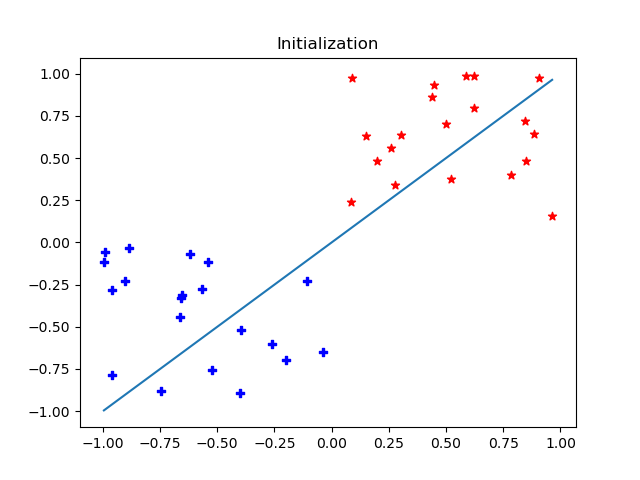
\includegraphics[scale=0.85]{init.png}
\end{figure}
It takes 1 iteration to converge and the corresponding figure is shown below:
\begin{figure}[!ht]
	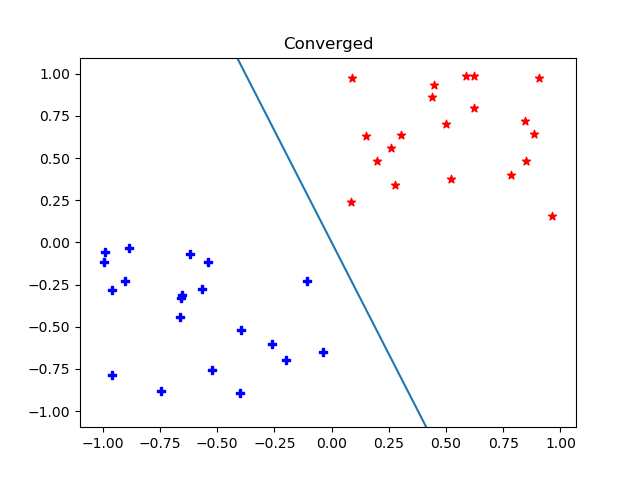
\includegraphics[scale=0.85]{converged.png}
\end{figure}
\newpage
\subsection*{Solution 3.2}
In this case, as the classes are not linearly separable, perceptron algorithm will not converge. The perceptron algorithm iterates till all the points are classified correctly by a linear decision boundary. But in case of linearly non-separable classes, there is no linear decision boundary which separates all the points correctly. After using a 'soft' linear classifier to tolerate error, we get the following plot:
\begin{figure}[!ht]
	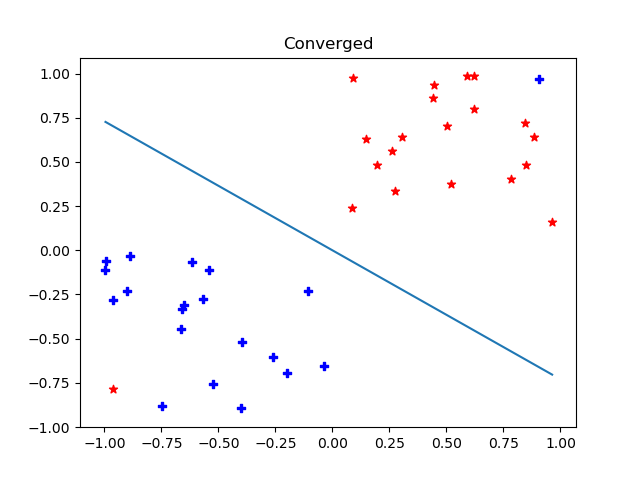
\includegraphics[scale=0.85]{problem3.png}
\end{figure}